% Provenance (never printed): see sources/outline_sources.md (Year 2: effusive and explosive
% eruptions, eruptive styles, eruption columns, pyroclastic deposits, explosivity index,
% volcano monitoring).
% Curves from figdata/bachelor-2/eruptions.py (closed-system gas fraction, Cotopaxi Layer 5
% thinning, GVP frequency-size law, column height fits, Mogi uplift); exercise and problem
% values in the Book 4 scratch calculators calc/ch06.py and calc/ch06pb.py.
\chapter{Vulkaanuitbarstingen}\label{ch:b2:eruptive-styles}

Op 15 juni 1991 wierp de Pinatubo, op de Filipijnen, meer dan vijf
kubieke kilometer materiaal uit; zijn aswolk steeg tot
\qty{35}{km}, de top stortte in tot een \omterm{def:b2:eruptive-styles:caldera}{caldera} van \qty{2.5}{km} doorsnede, en de
twintig miljoen ton zwaveldioxide die hij in de stratosfeer bracht, koelde de
hele aardbol twee jaar lang met ongeveer een halve graad af. Een week eerder had het eerste
\omterm{def:b2:magma-emplacement:magma}{magma} dat het oppervlak bereikte, niets van dat alles gedaan: het had onderweg het grootste deel van zijn
gas verloren en welde op als een \omterm{def:b2:eruptive-styles:dome}{lavakoepel}. Op Kīlauea, op Hawaï, stortte de
eruptie van Pu`u~`\=O`\=o \qty{4.4}{km^3} lava uit, vergelijkbaar in volume,
maar over vijfendertig jaar, als fonteinen en stromen die 215 gebouwen verwoestten
zonder ooit een torenhoge askolom op te bouwen. Dezelfde aarde, dezelfde fysica, drie gedragingen: wat
ze onderscheidt, is hoeveel gas een \omterm{def:b2:magma-emplacement:magma}{magma} meevoert, of dat gas de
smelt rustig kan verlaten, en hoe snel het \omterm{def:b2:magma-emplacement:magma}{magma} opstijgt. Dit hoofdstuk volgt een eruptie
van de bellen in het kanaal tot de kolom boven de krater en de afzettingen die ze
achterlaat, meet daarna erupties, telt ze, en bewaakt vulkanen op de
tekenen dat er een op komst is.
% ledger: usgs:pinatubo-1991, usgs:puuoo

\begin{recall}
\textbf{Uit de schoolboeken}: een vulkaan, zijn kraterpijp en krater, de
magmahaard eronder, lava en vulkanische as. \textbf{Uit
\cref{ch:b2:magma-emplacement}}: \omterm{def:b2:magma-emplacement:volatiles}{magmatische vluchtige bestanddelen}, hun ontmenging onder de
verzadigingsdruk, de wortelwet voor de oplosbaarheid van water $w = s\sqrt p$ met
$s \approx 0.34$ procent per $\sqrt{\unit{MPa}}$ voor basalt en $0.44$ voor
rhyoliet, en de viscositeiten van smelten, die tien grootteordes uiteenlopen.
\textbf{Uit de natuurkundeboeken}: de ideale gaswet $pV = nRT$; de opwaartse kracht;
dimensieanalyse, die de enige combinatie van gegeven grootheden opbouwt
die de dimensie van het antwoord heeft; de dracht van een projectiel, $v^2\sin 2\theta/g$
zonder luchtweerstand. \textbf{Uit de wiskundeboeken}: het poissonproces,
waarin onafhankelijke gebeurtenissen met een constante frequentie $\lambda$ minstens één gebeurtenis
in een tijd $t$ geven met kans $1 - e^{-\lambda t}$; kleinste-kwadratenrechten.
Uit Boek~3: aardbevingen en hun magnitudes.
\end{recall}

\section{Effusief of explosief}

\begin{definition}[Effusieve en explosieve erupties, fragmentatie]\label{def:b2:eruptive-styles:regimes}
Een \emph{effusieve eruptie}\index{effusieve eruptie} wordt beheerst door het
uitvloeien van lava, die als een samenhangende vloeistof van de krater wegstroomt. Een
\emph{explosieve eruptie}\index{explosieve eruptie} produceert vooral fragmenten,
as, puimsteen en ballistisch puin, meegevoerd door uitzettend gas. \emph{Fragmentatie
van magma}\index{fragmentatie van magma} is het uiteenvallen van een samenhangende smelt
met bellen tot een samenhangend gas dat druppels en fragmenten van de smelt meevoert;
ze maakt van een effusieve stroming een explosieve.
\end{definition}
% ledger: usgs:glossary-ch6, cassidy18:fragmentation

Wat de overgang aandrijft, is het gas. Een \omterm{def:b2:magma-emplacement:magma}{magma} dat uit de diepte opstijgt, voert
opgelost water en koolstofdioxide mee; onder zijn verzadigingsdruk komen de vluchtige bestanddelen
uit de oplossing vrij als bellen, en de bellen zetten uit naarmate de druk daalt.
Als ze in de smelt blijven, vult het gas al snel het grootste deel van het volume.

\begin{proposition}[Gasvolumefractie bij ontgassing in een gesloten systeem]\label{prop:b2:eruptive-styles:gas}
Laat een \omterm{def:b2:magma-emplacement:magma}{magma} een massafractie $w_0$ water bevatten, met oplosbaarheid $w(p) =
s\sqrt p$, en veronderstel dat het ontmengde water als ideaal gas bij temperatuur $T$
bij de smelt blijft. Onder de verzadigingsdruk $p_s = (w_0/s)^2$ bevat één
kilogram \omterm{def:b2:magma-emplacement:magma}{magma} $x = w_0 - s\sqrt p$ kilogram damp, en de
volumefractie gas is
\[
\phi(p) = \frac{V_g}{V_g + V_m}, \qquad V_g = \frac{x\,RT}{M p}, \qquad
V_m = \frac{1 - x}{\rho_m},
\]
waarbij $M = \qty{0.018}{kg/mol}$ de molaire massa van water is en $\rho_m$ de dichtheid
van de smelt.
\end{proposition}

\begin{proof}
Boven $p_s$ kan de smelt al zijn water bevatten en bestaat er geen gas. Onder $p_s$
houdt de smelt alleen zijn oplosbaarheid $s\sqrt p$, dus een massa $x = w_0 - s\sqrt p$ per
kilogram \omterm{def:b2:magma-emplacement:magma}{magma} is damp. Die damp, $x/M$ mol, neemt volgens de ideale gaswet $xRT/(Mp)$ in;
de resterende $1 - x$ kilogram smelt neemt $(1 - x)/\rho_m$ in.
De volumefractie volgt.
\end{proof}
% ledger: moore98:h2o

Omdat $V_g$ groeit als $1/p$, zwelt het schuim het snelst dicht bij het oppervlak. De
figuur hieronder volgt een rhyoliet met \qty{5}{\percent} water en een basalt
met \qty{1}{\percent}. Het rhyoliet raakt verzadigd bij \qty{127}{MPa}, ongeveer
\qty{5}{km} diep; bij \qty{10}{MPa} vult zijn gas al \qty{82}{\percent} van
het volume. In een gepubliceerd model van kanaalstroming fragmenteert het \omterm{def:b2:magma-emplacement:magma}{magma} wanneer het
gas \qty{85}{\percent} van zijn volume vult, een niveau dat dit rhyoliet bereikt bij
\qty{8.2}{MPa}, zo'n \qty{330}{m} onder de krater bij een drukgradiënt van
\qty{0.025}{MPa/m}. Het basalt raakt pas bij \qty{8.7}{MPa} verzadigd en bereikt
hetzelfde schuim bij \qty{1.8}{MPa}, binnen honderd meter van het oppervlak.
% ledger: cassidy18:fragmentation, cassidy18:ascent

\begin{omfigure}
\centering
\begin{tikzpicture}
\begin{axis}[omrecord, width=0.82\linewidth, height=5.6cm, xmode=log,
  xmin=0.01, xmax=200, ymin=0, ymax=1,
  xlabel={druk (\unit{MPa})}, ylabel={gasvolumefractie $\phi$},
  legend pos=south west, legend style={font=\scriptsize},
  tick label style={font=\scriptsize}, label style={font=\small}]
\addplot[very thick, red!70!black] table[x=p_MPa, y=rhyolite] {figdata/out/bachelor-2-eruptions-gas.dat};
\addlegendentry{rhyoliet, \qty{5}{\percent} H$_2$O, \qty{850}{\celsius}}
\addplot[very thick, black, dashed] table[x=p_MPa, y=basalt] {figdata/out/bachelor-2-eruptions-gas.dat};
\addlegendentry{basalt, \qty{1}{\percent} H$_2$O, \qty{1200}{\celsius}}
\draw[densely dotted, thick, gray] (axis cs:0.01,0.85) -- (axis cs:200,0.85);
\node[anchor=north west, font=\scriptsize, inner sep=1pt] at (axis cs:0.012,0.835) {fragmentatie in een kanaalmodel};
\end{axis}
\end{tikzpicture}
\par\smallskip{\small Volumefractie ontmengde waterdamp tegen de druk
bij ontgassing in een gesloten systeem (\cref{prop:b2:eruptive-styles:gas}), met de
oplosbaarheidswetten van \cref{ch:b2:magma-emplacement}. De druk daalt naar links, terwijl het \omterm{def:b2:magma-emplacement:magma}{magma}
opstijgt; de stippellijn markeert de gasfractie waarbij een gepubliceerd kanaalmodel
het \omterm{def:b2:magma-emplacement:magma}{magma} fragmenteert.}
\end{omfigure}
% ledger: moore98:h2o, cassidy18:fragmentation

Een basalt zou dus ook fragmenteren als zijn gas erin bleef; en in een Hawaïaanse
lavafontein gebeurt dat ook, dicht bij de krater. Wat de meeste basaltische erupties mild maakt, is dat
het gas niet hoeft te blijven. In een smelt met lage viscositeit stijgen bellen door de
vloeistof, versmelten en ontsnappen ze, en zodra bellen zich tot een doorlatend netwerk verbinden,
wat in experimenten gebeurt bij gasfracties tussen \qty{30}{\percent} en \qty{78}{\percent},
lekt het gas door de wanden en de krater weg zonder de
smelt mee te voeren: het \omterm{def:b2:magma-emplacement:magma}{magma} ontgast in een open systeem en bereikt het oppervlak als
lava. Een viskeus \omterm{def:b2:magma-emplacement:magma}{magma} houdt zijn bellen vast en fragmenteert in plaats daarvan; de smelt breekt
als glas wanneer hij sneller wordt uitgerekt dan hij kan vloeien. De opstijgsnelheid beslist
evenveel tussen de twee als de samenstelling: over veel erupties gaat effusieve activiteit
samen met decompressiesnelheden rond \qty{0.0001}{MPa/s} en gaan \omterm{def:b2:eruptive-styles:regimes}{explosieve erupties}
samen met snelheden rond \qty{1}{MPa/s}, en een verandering van de viscositeit van de smelt met een halve
logaritmische eenheid, ongeveer een factor drie, kan een eruptie van het ene regime naar
het andere doen omslaan. De eerste \omterm{def:b2:eruptive-styles:dome}{lavakoepel} van de Pinatubo en zijn hoofderuptie een week later
waren hetzelfde \omterm{def:b2:magma-emplacement:magma}{magma}: de eerste portie had tijd om haar gas te verliezen, de volgende niet.
% ledger: cassidy18:fragmentation, cassidy18:ascent, usgs:pinatubo-1991

Water van buitenaf doet wat het eigen gas van het \omterm{def:b2:magma-emplacement:magma}{magma} doet. Grondwater, een meer of de
zee die \omterm{def:b2:magma-emplacement:magma}{magma} ontmoet, verdampt in een flits, en de uitzetting van het oververhitte
water verbrijzelt het \omterm{def:b2:magma-emplacement:magma}{magma}: experimenten tonen dat meer dan \qty{30}{\percent} van
de beschikbare warmte in mechanische energie kan worden omgezet. Zelfs gasarm \omterm{def:b2:magma-emplacement:magma}{magma}
kan dan explosief uitbarsten.
% ledger: cassidy18:fragmentation

\section{Eruptiestijlen}

Vulkanologen noemen erupties naar klassieke voorbeelden. De namen beschrijven hoe een
eruptie eruitziet, en ze gaan geleidelijk in elkaar over; één eruptie doorloopt vaak
meerdere stijlen.

\begin{definition}[Eruptiestijlen]\label{def:b2:eruptive-styles:styles}
In volgorde van toenemende explosiviteit, onder de erupties die door het eigen gas van het \omterm{def:b2:magma-emplacement:magma}{magma} worden aangedreven:
\begin{itemize}
\item een \emph{Hawaïaanse eruptie}\index{Hawaïaanse eruptie} produceert fonteinen van
zeer vloeibare basaltlava, tientallen tot honderden meters hoog, die lavastromen voeden;
\item een \emph{Strombolische eruptie}\index{Strombolische eruptie} is een reeks
afzonderlijke uitbarstingen die gloeiende klonten basaltisch tot
basaltisch-andesitisch \omterm{def:b2:magma-emplacement:magma}{magma} tot ongeveer honderd meter hoog werpen, zonder aanhoudende
kolom;
\item een \emph{Vulcanische eruptie}\index{Vulcanische eruptie} is een korte, hevige
explosie van gas dat zich onder een prop gestolde lava heeft opgehoopt, die
de prop verbrijzelt en blokken en een donkere kolom fijne as uitwerpt, meestal uit
intermediair \omterm{def:b2:magma-emplacement:magma}{magma};
\item een \emph{Plinische eruptie}\index{Plinische eruptie} is een aanhoudende straal van gas
en gefragmenteerd, meestal silicarijk, \omterm{def:b2:magma-emplacement:magma}{magma} die een kolom voedt die urenlang tot dagenlang tot in de
stratosfeer stijgt en een laag puimsteen en as verspreidt over
duizenden vierkante kilometer.
\end{itemize}
Waar water van buitenaf de fragmentatie aandrijft, werpt een \emph{freatomagmatische
eruptie}\index{freatomagmatische eruptie} stoom uit samen met fragmenten
van vers \omterm{def:b2:magma-emplacement:magma}{magma}, terwijl een \emph{freatische eruptie}\index{freatische eruptie} een
door stoom aangedreven explosie is van grond- of oppervlaktewater dat door \omterm{def:b2:magma-emplacement:magma}{magma} of heet gesteente is verhit,
die stoom en fragmenten van ouder gesteente uitwerpt, maar geen vers \omterm{def:b2:magma-emplacement:magma}{magma}.
\end{definition}
% ledger: nps:styles, usgs:glossary-ch6

Elke stijl heeft zijn type-erupties. Pu`u~`\=O`\=o, op Kīlauea, was Hawaïaans gedurende het grootste deel van
zijn vijfendertig jaar en eenenzestig episoden, met fonteinen die gewoonlijk
\qtyrange{10}{100}{m} hoog werden en soms meer dan \qty{500}{m}. Stromboli, de
``vuurtoren van de Middellandse Zee'', heeft zijn naam gegeven aan de uitbarstingen die
sintelkegels opbouwen. Vulcanische explosies deden Trident in Alaska met tussenpozen beven tussen
1953 en 1974. De Vesuvius in 79 n.Chr., beschreven door Plinius de Jongere, gaf zijn naam aan
de \omterm{def:b2:eruptive-styles:styles}{Plinische erupties}; Mount St.~Helens op 18~mei~1980 en Novarupta in 1912, waarvan de
kolom boven \qty{30}{km} uitsteeg in een eruptie die bijna drie dagen duurde, zijn
moderne voorbeelden.
Tussengevallen met kolommen onder ongeveer \qty{20}{km}, aanhoudend maar onregelmatig,
heten sub-Plinisch. Met water wordt een \omterm{def:b2:eruptive-styles:styles}{Strombolische eruptie} Surtseyaans,
naar de eruptie van Surtsey in 1963 voor de kust van IJsland, en bouwt ze lage
tufringen en maren op; een Plinische wordt freatoplinisch. Bij de Pinatubo bliezen
stoomexplosies in maart en april 1991 drie kraters in de noordflank, twee
maanden voor de hoofderuptie: ze waren freatisch.
% ledger: nps:styles, usgs:puuoo, usgs:glossary-ch6, usgs:pinatubo-deposits

\begin{definition}[Lavakoepel]\label{def:b2:eruptive-styles:dome}
Een \emph{lavakoepel}\index{lavakoepel} is een steile heuvel van viskeuze lava,
meestal daciet of rhyoliet, die langzaam uit een krater wordt geperst en zich erboven ophoopt
in plaats van weg te stromen.
\end{definition}
% ledger: usgs:glossary-ch6

Koepels zijn wat een viskeus \omterm{def:b2:magma-emplacement:magma}{magma} vormt wanneer het zijn gas heeft verloren: het eerste
\omterm{def:b2:magma-emplacement:magma}{magma} van de Pinatubo in juni 1991, en de koepel die in de krater van Mount St.~Helens in
zeventien episoden tussen 1980 en 1986 groeide tot \qty{267}{m} boven de kraterbodem.
Een koepel kan ook de prop zijn waaronder de volgende Vulcanische explosie zich opbouwt,
en zijn instorting kan de druk wegnemen van het gasrijke \omterm{def:b2:magma-emplacement:magma}{magma} eronder. De
foto's hieronder tonen de twee uitersten van het bereik.
% ledger: usgs:pinatubo-1991, usgs:msh-dome, cassidy18:fragmentation

\begin{omfigure}
\centering
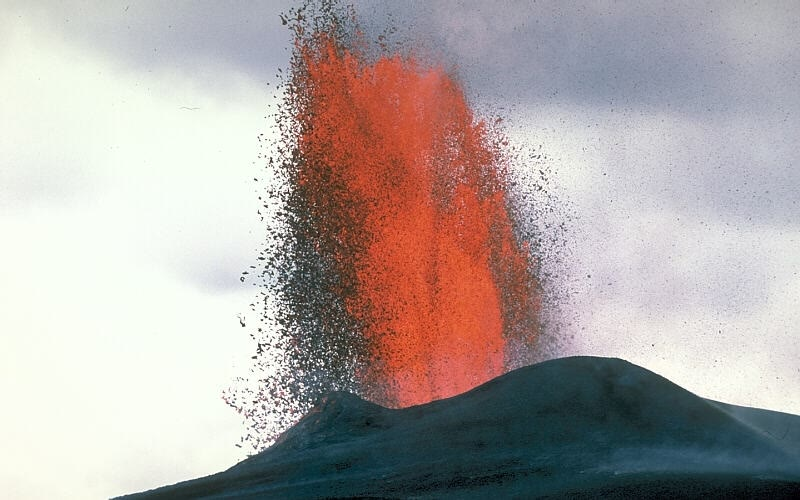
\includegraphics[height=4.3cm]{images/book4/b2-kilauea-fountain.jpg}\hfill
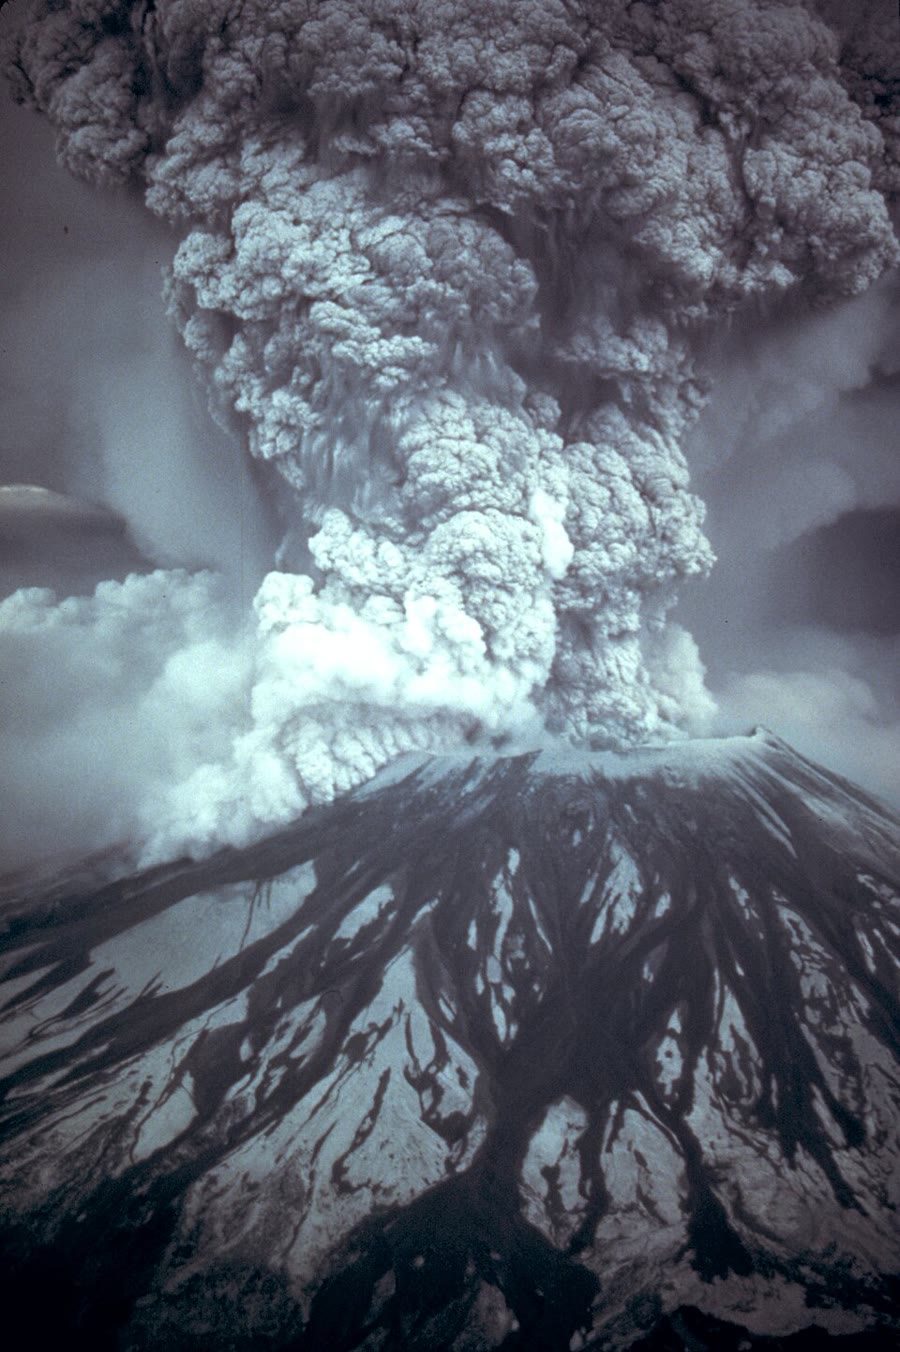
\includegraphics[height=4.3cm]{images/book4/b2-st-helens-column.jpg}\hfill
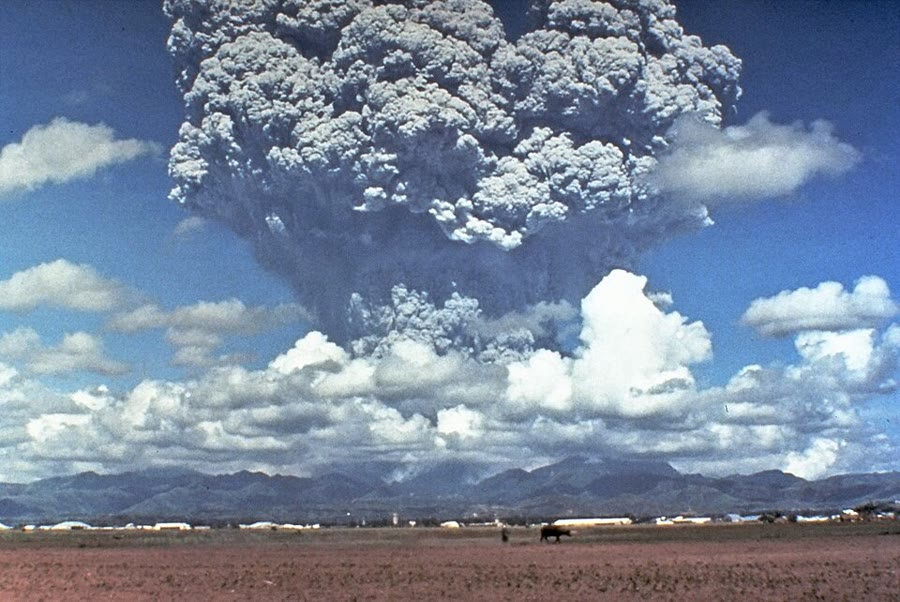
\includegraphics[height=4.3cm]{images/book4/b2-pinatubo-column.jpg}
\par\smallskip{\small Links: een Hawaïaanse fontein op de kegel Pu`u~`\=O`\=o van Kīlauea,
oktober 1983 (J.\,D.~Griggs, USGS). Midden: de Plinische kolom van Mount St.~Helens,
18 mei 1980 (Austin Post, USGS). Rechts: de \omterm{def:b2:eruptive-styles:column}{eruptiekolom} van de Pinatubo op
12 juni 1991, drie dagen voor de hoofderuptie (Dave Harlow, USGS). Alle
drie de foto's zijn publiek domein.}
\end{omfigure}
% ledger: usgs:puuoo, usgs:msh-may18, usgs:pinatubo-1991

\section{Eruptiekolommen}

\begin{definition}[Eruptiekolom]\label{def:b2:eruptive-styles:column}
Een \emph{eruptiekolom}\index{eruptiekolom} is de opstijgende massa gas en
fragmenten boven een explosieve krater. Ze heeft drie delen: een \emph{straal}, of
gasstuwzone, waarin het mengsel de krater snel maar dichter dan de
lucht verlaat en door zijn impuls stijgt; een \emph{convectieve} zone, waarin het mengsel,
dat genoeg lucht heeft opgeslokt en verhit om lichter te worden dan zijn omgeving,
door opwaartse kracht stijgt; en een \emph{paraplu}wolk, die zich zijwaarts uitspreidt op het
niveau waar de dichtheid van de kolom gelijk is aan die van de atmosfeer.
\end{definition}
% ledger: usgs:glossary-ch6, nps:styles, aubry23:fits

\begin{omfigure}
\centering
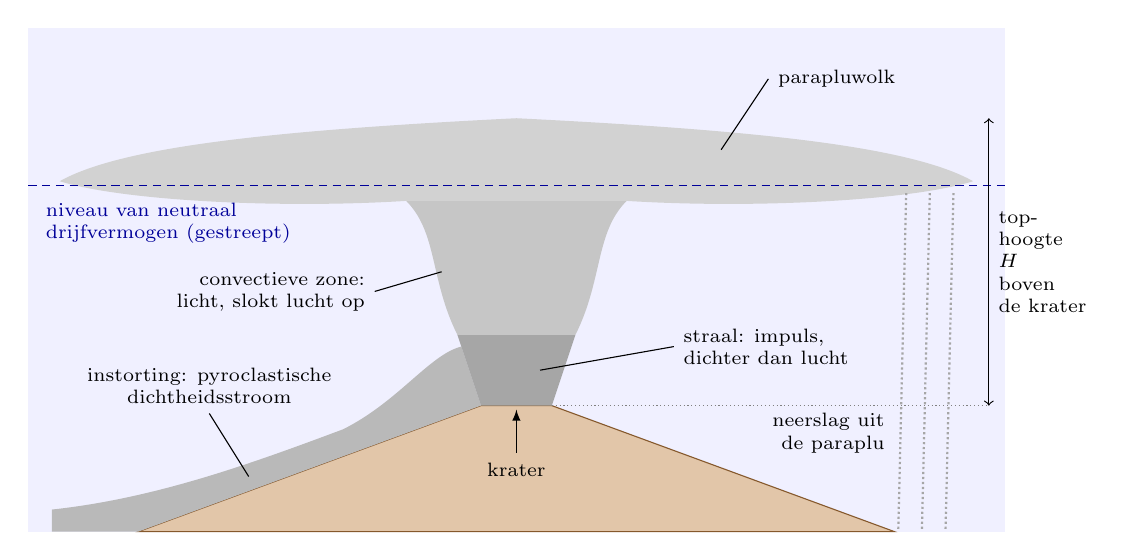
\begin{tikzpicture}[x=1cm, y=1cm, font=\scriptsize]
% atmosphere and ground
\fill[blue!6] (-6.2,0) rectangle (6.2,6.4);
% volcano
\fill[brown!45, draw=brown!70!black] (-4.8,0) -- (-0.45,1.6) -- (0.45,1.6) -- (4.8,0) -- cycle;
% collapse branch (left): a density current hugging the flank
\fill[gray!55] (-0.45,1.6) -- (-0.7,2.35) .. controls (-1.1,2.25) and (-1.5,1.65) .. (-2.2,1.3)
  .. controls (-3.4,0.85) and (-4.6,0.42) .. (-5.9,0.28) -- (-5.9,0) -- (-4.8,0) -- cycle;
% jet
\fill[gray!70] (-0.45,1.6) -- (0.45,1.6) -- (0.75,2.5) -- (-0.75,2.5) -- cycle;
% convective column
\fill[gray!45] (-0.75,2.5) .. controls (-1.1,3.2) and (-1.0,3.8) .. (-1.4,4.2)
  -- (1.4,4.2) .. controls (1.0,3.8) and (1.1,3.2) .. (0.75,2.5) -- cycle;
% umbrella
\fill[gray!35] (-1.4,4.2) .. controls (-3,4.1) and (-5,4.2) .. (-5.8,4.45)
  .. controls (-5,4.9) and (-3,5.1) .. (0,5.25) .. controls (3,5.1) and (5,4.9) .. (5.8,4.45)
  .. controls (5,4.2) and (3,4.1) .. (1.4,4.2) -- cycle;
\draw[densely dashed, blue!60!black] (-6.2,4.4) -- (6.2,4.4);
% fallout from the far end of the umbrella, down to the ground
\foreach \x in {4.95,5.25,5.55} {\draw[gray!70, densely dotted, thick] (\x,4.3) -- (\x-0.1,0.02);}
\draw[gray, densely dotted] (0.45,1.6) -- (6.0,1.6);
\draw[<->] (6.0,1.6) -- (6.0,5.25) node[midway, right, align=left] {top-\\hoogte\\$H$\\boven\\de krater};
% labels
\node[anchor=north west, align=left, blue!60!black] at (-6.1,4.3) {niveau van neutraal\\drijfvermogen (gestreept)};
\draw (-0.95,3.3) -- (-1.8,3.05) node[left, align=right] {convectieve zone:\\licht, slokt lucht op};
\draw (0.3,2.05) -- (2.0,2.35) node[right, align=left] {straal: impuls,\\dichter dan lucht};
\draw (2.6,4.85) -- (3.2,5.75) node[right] {parapluwolk};
\node[anchor=east, align=right] at (4.8,1.25) {neerslag uit\\de paraplu};
\draw (-3.4,0.7) -- (-3.9,1.5) node[above, align=center] {instorting: pyroclastische\\dichtheidsstroom};
\draw[-latex] (0,1.0) -- (0,1.55);
\node[anchor=north] at (0,1.0) {krater};
\end{tikzpicture}
\par\smallskip{\small Bouw van een \omterm{def:b2:eruptive-styles:column}{eruptiekolom} (schematisch, niet op schaal). Rechts
stijgt de kolom door zijn drie zones en laat de parapluwolk
\omterm{def:b2:eruptive-styles:tephra}{tefra} vallen terwijl ze zich uitspreidt; links is een deel van de straal er niet in geslaagd
licht te worden en stort het in tot een \omterm{def:b2:eruptive-styles:pdc}{pyroclastische dichtheidsstroom}.}
\end{omfigure}

Hoe hoog een kolom stijgt, hangt vooral af van hoeveel warmte ze per
seconde aanvoert, dat wil zeggen van het massadebiet van de eruptie~$Q$. Dimensieanalyse geeft de
vorm van de wet.

\begin{proposition}[Hoogte van een lichte pluim]\label{prop:b2:eruptive-styles:plume}
Als de tophoogte $H$ van een lichte pluim boven een stationaire puntbron alleen afhangt
van de opwaartse flux $F$ van de bron (dimensie $\mathrm{m^4\,s^{-3}}$) en van de
brunt-väisäläfrequentie $N$ van een stabiel gelaagde atmosfeer (dimensie
$\mathrm{s^{-1}}$), dan geldt
\[
H = c\,F^{1/4}N^{-3/4}
\]
met $c$ een dimensieloze constante. Omdat $F$ evenredig is met de warmteflux, en dus
met het massadebiet van de eruptie, geldt $H \propto Q^{1/4}$ in een gegeven atmosfeer.
\end{proposition}

\begin{proof}
Schrijf $H = c\,F^{\alpha}N^{\beta}$. Gelijkstellen van de lengten geeft $4\alpha = 1$; gelijkstellen van de
tijden geeft $-3\alpha - \beta = 0$. Dus $\alpha = 1/4$ en $\beta = -3/4$, en geen
andere combinatie van $F$ en $N$ heeft de dimensie van een lengte.
\end{proof}

De constante $c$ komt van hoe snel de pluim lucht opslokt, wat de pluimtheorie
behandelt met een meesleurcoëfficiënt die in experimenten wordt gemeten; ze wordt hier
aangenomen. Echte kolommen zijn geen stationaire puntbronnen in een windstille atmosfeer, dus
vulkanologen fitten de wet op erupties waarvan hoogte en massadebiet
allebei zijn gemeten.
% ledger: aubry23:fits

\begin{proposition}[Kolomhoogte en massadebiet van de eruptie]\label{prop:b2:eruptive-styles:mastin}
Voor de tophoogte $H$ boven de krater in kilometer en het massadebiet van de eruptie
$Q$ in kilogram per seconde geeft de compilatie van goed gedocumenteerde erupties
\[
H = 0.304\,Q^{0.241},
\]
en een grotere, onafhankelijke gegevensreeks van 130 gebeurtenissen geeft $H = 0.345\,Q^{0.226}$.
De spreiding is groot: de relatieve wortel-gemiddelde-kwadratische fout op $H$ is
\qtyrange{53}{60}{\percent}.
\end{proposition}
\admitted
% ledger: aubry23:fits

Beide exponenten liggen dicht bij de $1/4$ van de pluimtheorie. De figuur hieronder toont
de twee fits en de voorbeelderupties waarop de bronparameters van
centra voor asvoorspelling berusten. Een kolom van \qty{15}{km} hoog, zoals die van Mount
St.~Helens, vraagt \qty{e7}{kg/s}, tienduizend ton per seconde; een verdubbeling van de
hoogte vraagt bijna achttien keer het debiet. Omgekeerd gelezen geeft een gemeten hoogte
het debiet, maar slechts tot op een factor van enkele nauwkeurig, omdat $Q$ gaat als $H^4$
(\cref{exo:b2:eruptive-styles:3}). Vulkanologen drukken het debiet uit met de \emph{intensiteit} $I =
\log_{10}Q + 3$, met $Q$ in kilogram per seconde.
% ledger: mastin09:examples, aubry23:fits, brown14:record

\begin{omfigure}
\centering
\begin{tikzpicture}
\begin{axis}[omrecord, width=0.82\linewidth, height=6cm, xmode=log, ymode=log,
  xmin=1e3, xmax=1e9, ymin=1, ymax=60,
  xlabel={massadebiet van de eruptie $Q$ (\unit{kg/s})}, ylabel={tophoogte boven de krater (\unit{km})},
  ytick={1,2,5,10,20,50}, yticklabels={1,2,5,10,20,50},
  legend pos=north west, legend style={font=\scriptsize},
  tick label style={font=\scriptsize}, label style={font=\small}]
\addplot[very thick, black] table[x=Q, y=mastin] {figdata/out/bachelor-2-eruptions-column.dat};
\addlegendentry{$H = 0.304\,Q^{0.241}$}
\addplot[thick, red!70!black, dashed] table[x=Q, y=aubry] {figdata/out/bachelor-2-eruptions-column.dat};
\addlegendentry{$H = 0.345\,Q^{0.226}$}
\addplot[only marks, mark=*, mark size=1.8pt, blue!70!black]
  table[x=Q, y=H] {figdata/out/bachelor-2-eruptions-column-data.dat};
\addlegendentry{voorbeelderupties}
\begin{scope}[font=\tiny, inner sep=1.5pt]
\node[anchor=north west] at (axis cs:5e3,2) {Etna 2001};
\node[anchor=south east] at (axis cs:1e5,7) {Cerro Negro 1992};
\node[anchor=north west] at (axis cs:2e5,5) {Ruapehu 1996};
\node[anchor=east] at (axis cs:1e6,10) {Fuego 1974};
\draw[gray] (axis cs:3e6,10) -- (axis cs:2e7,4.5) node[anchor=west, black] {Soufrière Hills};
\draw[gray] (axis cs:4e6,11) -- (axis cs:2e7,6.5) node[anchor=west, black] {Spurr 1992};
\node[anchor=south east] at (axis cs:1e7,15) {St Helens 1980};
\node[anchor=south east, align=right] at (axis cs:1e8,25) {St Helens\\co-ignimbriet};
\end{scope}
\end{axis}
\end{tikzpicture}
\par\smallskip{\small Tophoogte van eruptiekolommen boven de krater tegen het
massadebiet van de eruptie: de empirische fit van Mastin en anderen (2009), de fit van
Aubry en anderen (2023) op een onafhankelijke gegevensreeks, en de voorbeelderupties
van de eerste compilatie (de co-ignimbrietwolk van Mount St.~Helens steeg op uit
\omterm{def:b2:eruptive-styles:pdc}{pyroclastische stromen}, niet uit de krater).}
\end{omfigure}
% ledger: aubry23:fits, mastin09:examples

Een kolom kan er ook niet in slagen te stijgen. De straal verlaat de krater dichter dan lucht; als hij
zijn impuls verliest voordat hij genoeg lucht heeft opgeslokt om licht te worden,
bijvoorbeeld omdat zijn gasgehalte daalt, stort de kolom in en stroomt het mengsel
als een hete, dichte stroom langs de flanken omlaag. Plinische kolommen kunnen op
deze manier instorten, en bij de Pinatubo vulden de \omterm{def:b2:eruptive-styles:pdc}{pyroclastische stromen} van 1991 dalen met
afzettingen tot \qty{200}{m} dik.
% ledger: nps:styles, usgs:pinatubo-deposits

\section{Pyroclastische producten}

\begin{definition}[Tefra en pyroclasten]\label{def:b2:eruptive-styles:tephra}
Een \emph{pyroclast}\index{pyroclast} is een fragment dat ontstaat door de explosieve
\omterm{def:b2:eruptive-styles:regimes}{fragmentatie van magma} of van de gesteenten eromheen. \emph{Tefra}\index{tefra} is
de verzamelnaam van alle pyroclasten die in de lucht worden geworpen, wat hun grootte ook is.
Naar grootte vormen pyroclasten fijner dan \qty{2}{mm} vulkanische as; die van
\qtyrange{2}{64}{mm} zijn \emph{lapilli}\index{lapilli}; die groter dan
\qty{64}{mm} zijn blokken als ze vast en hoekig waren bij het uitwerpen, en een
\emph{vulkanische bom}\index{vulkanische bom} als ze geheel of gedeeltelijk gesmolten waren
en tijdens de vlucht een ronde of spoelvorm aannamen.
\end{definition}
% ledger: nps:pyroclast-sizes, usgs:glossary-ch6

\omterm{def:b2:eruptive-styles:tephra}{Tefra} valt uit de parapluwolk en de kolom met de wind mee als een valafzetting
die het land bedekt: dik dicht bij de krater, dunner en fijner verder weg. Haar
dikte wordt in kaart gebracht met \emph{isopachen}, lijnen van gelijke dikte, en neemt in de regel
exponentieel af met de afstand. Omdat de wind de isopachen
tot ellipsen uitrekt, wordt de afstand het best gemeten met de vierkantswortel van de oppervlakte die elke
isopach omsluit.
% ledger: usgs:ash-props, biass19:layer5

\begin{proposition}[Volume van een exponentieel dunner wordende afzetting]\label{prop:b2:eruptive-styles:thinning}
Als de dikte van een valafzetting afneemt met de vierkantswortel $x = \sqrt A$
van de isopachoppervlakte als $T = T_0\,e^{-kx}$, is haar bulkvolume
\[
V = \frac{2T_0}{k^2}.
\]
De helft van dat volume ligt voorbij de isopach $x_{1/2} = 1.678/k$.
\end{proposition}

\begin{proof}
Tussen de isopachen met oppervlakten $A$ en $A + dA$ heeft de afzetting het volume $T\,dA$,
en $dA = 2x\,dx$. Dus $V = \int_0^\infty T_0e^{-kx}\,2x\,dx = 2T_0/k^2$, door
partiële integratie ($\int_0^\infty xe^{-kx}dx = 1/k^2$). Het volume binnen $x$
is $\frac{2T_0}{k^2}[1 - (1 + kx)e^{-kx}]$, wat de helft van het totaal is als $(1 +
u)e^{-u} = 1/2$ met $u = kx$, dat wil zeggen $u = 1.678$.
\end{proof}

Echte afzettingen worden dunner met twee of meer hellingen, steil dicht bij de krater en flauw ver
weg, omdat de grove \omterm{def:b2:eruptive-styles:tephra}{lapilli} snel uit de kolom vallen en de fijne as
wegdrijft. Elk segment wordt afzonderlijk gefit en de integraal wordt stuk voor
stuk genomen.

\begin{method}[Volume van een valafzetting uit haar isopachen]\label{met:b2:eruptive-styles:volume}
Zet $\ln T$ uit tegen $\sqrt A$ voor elke isopach en fit een rechte lijn door elke
reeks punten die op één lijn liggen. Voor twee segmenten, $T_0e^{-k_1x}$ binnen het snijpunt
$X$ van de twee lijnen en het tweede segment erbuiten, is het volume
\[
V = \frac{2T_0}{k_1^2} + 2T_0e^{-k_1X}\left[\frac{k_2X + 1}{k_2^2} -
\frac{k_1X + 1}{k_1^2}\right]
\]
(\cref{exo:b2:eruptive-styles:10}). Reken het bulkvolume om naar een equivalent in dicht gesteente, het volume van
dezelfde massa als \omterm{def:b2:magma-emplacement:magma}{magma} zonder bellen, met $V_{\mathrm{DRE}} = V\rho_{\mathrm{deposit}}/\rho_{\mathrm{magma}}$.
\end{method}
% ledger: biass19:layer5, brown14:record

De figuur hieronder past de methode toe op een slakkenvalafzetting van de Cotopaxi, in
Ecuador, van ongeveer \num{1200} jaar geleden. Twee segmenten passen bij de zes isopachen, met
halveringsafstanden van de dikte $\ln 2/k$ van \qty{1.9}{km} en \qty{5.0}{km} (de
gepubliceerde studie, waarvan de fit iets verschilt, vindt \qty{1.9}{km} en
\qty{5.3}{km}), en het volume komt uit op \qty{0.29}{km^3}, zoals in die studie. Meer dan
\qty{40}{\percent} ervan ligt in het dunne distale segment, en daarom weegt distale as,
die gemakkelijk wegerodeert of nooit in kaart wordt gebracht, zo zwaar in het totaal. Vers gevallen as
heeft een bulkdichtheid van \qtyrange{500}{1500}{kg/m^3}, ver onder die van het
\omterm{def:b2:magma-emplacement:magma}{magma}, dus het equivalent in dicht gesteente is ruwweg de helft van het bulkvolume of minder.
% ledger: biass19:layer5, usgs:ash-props

\begin{omfigure}
\centering
\begin{tikzpicture}
\begin{axis}[omrecord, width=0.78\linewidth, height=5.6cm, ymode=log,
  xmin=0, xmax=30, ymin=2, ymax=2000,
  xlabel={$\sqrt{\text{isopachoppervlakte}}$ (\unit{km})}, ylabel={dikte (\unit{cm})},
  ytick={2,5,10,20,50,100,200,500,1000,2000}, yticklabels={2,5,10,20,50,100,200,500,1000,2000},
  legend pos=north east, legend style={font=\scriptsize},
  tick label style={font=\scriptsize}, label style={font=\small}]
\addplot[thick, black, restrict x to domain=0:12] table[x=sqrtA_km, y=seg1] {figdata/out/bachelor-2-eruptions-thin-fit.dat};
\addlegendentry{proximaal segment, $k_1 = \qty{0.365}{km^{-1}}$}
\addplot[thick, red!70!black, dashed, restrict x to domain=5:30] table[x=sqrtA_km, y=seg2] {figdata/out/bachelor-2-eruptions-thin-fit.dat};
\addlegendentry{distaal segment, $k_2 = \qty{0.138}{km^{-1}}$}
\addplot[only marks, mark=*, mark size=2pt, blue!70!black] table[x=sqrtA_km, y=T_cm] {figdata/out/bachelor-2-eruptions-thin-data.dat};
\addlegendentry{isopachen}
\end{axis}
\end{tikzpicture}
\par\smallskip{\small Dunner worden van de slakkenvalafzetting Laag~5 van de Cotopaxi (Ecuador),
ongeveer \num{1200} jaar oud: diktes van de isopachen volgens Biass, Bonadonna en
Houghton (2019) tegen de vierkantswortel van de oppervlakte die elke isopach omsluit (de
verticale schaal is logaritmisch). Twee exponentiële segmenten, gefit op de twee
proximale en de vier distale isopachen, snijden elkaar bij $\sqrt A = \qty{8.6}{km}$;
geïntegreerd geven ze een bulkvolume van \qty{0.29}{km^3}.}
\end{omfigure}
% ledger: biass19:layer5

Niet alle \omterm{def:b2:eruptive-styles:tephra}{tefra} valt uit de lucht. Wanneer een kolom instort, een koepel afbrokkelt of een
zijwaartse explosie de flank van een vulkaan openscheurt, loopt het hete mengsel over de
grond.

\begin{definition}[Pyroclastische dichtheidsstromen]\label{def:b2:eruptive-styles:pdc}
Een \emph{pyroclastische dichtheidsstroom}\index{pyroclastische dichtheidsstroom} is een
mengsel van heet gas en \omterm{def:b2:eruptive-styles:tephra}{pyroclasten} dat langs de grond hellingafwaarts of naar buiten stroomt
omdat het dichter is dan de lucht. Een \emph{pyroclastische stroom}\index{pyroclastische stroom} is een geconcentreerde stroom van gesteentefragmenten, as en gas, meestal van
\qtyrange{200}{700}{\celsius}, die met tientallen meters per seconde beweegt; een
\emph{pyroclastische golf}\index{pyroclastische golf} is een ijlere wolk van as,
gesteente en gas, van enkele honderden graden, die met de snelheid van een
orkaanwind beweegt. Een \emph{ignimbriet}\index{ignimbriet} is het gesteente dat door pyroclastische
dichtheidsstromen is afgezet en dat door zijn eigen warmte kan zijn samengelast.
\end{definition}
% ledger: usgs:glossary-ch6

Op 18 mei 1980 legde de instorting van de noordflank van Mount St.~Helens, de grootste
aardverschuiving in de opgetekende geschiedenis met ongeveer \qty{2.8}{km^3}, het \omterm{def:b2:magma-emplacement:magma}{magma} bloot en
ontketende ze een zijwaartse explosie die ongeveer \qty{600}{km^2} doorkruiste met tot
\qty{480}{km/h}; \omterm{def:b2:eruptive-styles:pdc}{pyroclastische stromen} van minstens \qty{700}{\celsius} bereikten daarna
\qty{8}{km} van de krater. De stromen van de Pinatubo van 1991 waren vijf jaar later vanbinnen nog
\qty{500}{\celsius} heet.
% ledger: usgs:msh-may18, usgs:msh-flows, usgs:msh-reach, usgs:pinatubo-deposits

\begin{definition}[Lahar]\label{def:b2:eruptive-styles:lahar}
Een \emph{lahar}\index{lahar} is een snel bewegend mengsel van water en vulkanisch puin
dat door een rivierdal stroomt, met een consistentie die varieert van modderig water
tot nat beton. Lahars ontstaan wanneer \omterm{def:b2:eruptive-styles:pdc}{pyroclastische stromen} sneeuw en ijs doen smelten, wanneer
zware regen op losse vulkanische afzettingen valt, wanneer een meer dat door vulkanische
afzettingen is afgedamd doorbreekt, of uit een puinlawine.
\end{definition}
% ledger: usgs:glossary-ch6

\omterm{def:b2:eruptive-styles:lahar}{Lahars} duren langer dan erupties. Rond de Pinatubo maakten moesson- en tyfoonregens
van de as van 1991 jarenlang \omterm{def:b2:eruptive-styles:lahar}{lahars}, en die richtten meer verwoesting aan dan de
eruptie zelf.
% ledger: usgs:pinatubo-lahars

\begin{definition}[Caldera]\label{def:b2:eruptive-styles:caldera}
Een \emph{caldera}\index{caldera} is een grote komvormige vulkanische depressie,
\qtyrange{2}{50}{km} breed en veel breder dan elke krater erin, gevormd door
het instorten van de bodem in een ondiep magmareservoir dat een eruptie
gedeeltelijk heeft leeggemaakt.
\end{definition}
% ledger: usgs:glossary-ch6

De \omterm{def:b2:eruptive-styles:caldera}{caldera}'s van de Pinatubo en van Novarupta hebben beide een doorsnede van ongeveer \qty{2.5}{km}, aan de
kleine kant van het bereik. Een \omterm{def:b2:eruptive-styles:caldera}{caldera} verschilt van een krater, die kleiner is en door explosies is uitgegraven.
% ledger: usgs:pinatubo-1991, nps:styles, usgs:glossary-ch6

\section{Erupties meten en tellen}

\begin{definition}[Vulkanische explosiviteitsindex]\label{def:b2:eruptive-styles:vei}
De \emph{vulkanische explosiviteitsindex}\index{vulkanische explosiviteitsindex} (VEI) is
een geheel getal van 0 tot 8 dat de grootte van een eruptie meet, vooral via het
bulkvolume van haar \omterm{def:b2:eruptive-styles:tephra}{tefra}: VEI~0 voor minder dan \qty{e4}{m^3}, VEI~1 tot
\qty{e6}{m^3}, daarna één stap per factor tien, tot VEI~8 boven
\qty{e12}{m^3}, \qty{1000}{km^3}. Kolomhoogte en beschrijvingen van de eruptie
worden gebruikt als het volume niet bekend is. Een niet-explosieve eruptie heeft VEI~0,
wat het volume van haar lava ook is.
\end{definition}
% ledger: usgs:vei-criteria, usgs:msh-comparisons

\begin{table}[ht]
\centering
\small
\begin{tabular}{llll}
\hline
VEI & bulkvolume \omterm{def:b2:eruptive-styles:tephra}{tefra} (\unit{m^3}) & kolomhoogte (\unit{km}) & gebruikelijke stijl \\
\hline
0 & $< 10^{4}$ & $< 0.1$ & Hawaïaans \\
1 & $10^{4}$--$10^{6}$ & 0.1--1 & Hawaïaans, Strombolisch \\
2 & $10^{6}$--$10^{7}$ & 1--5 & Strombolisch, Vulcanisch \\
3 & $10^{7}$--$10^{8}$ & 3--15 & Vulcanisch \\
4 & $10^{8}$--$10^{9}$ & 10--25 & Vulcanisch, Plinisch \\
5 & $10^{9}$--$10^{10}$ & $> 25$ & Plinisch \\
6 & $10^{10}$--$10^{11}$ & $> 25$ & Plinisch \\
7 & $10^{11}$--$10^{12}$ & $> 25$ & Plinisch \\
8 & $> 10^{12}$ & $> 25$ & Plinisch \\
\hline
\end{tabular}
\caption{Criteria van de \omterm{def:b2:eruptive-styles:vei}{vulkanische explosiviteitsindex} (naar Newhall en Self, 1982).}
\label{tab:b2:eruptive-styles:vei}
\end{table}
% ledger: usgs:vei-criteria

De index is logaritmisch zoals een aardbevingsmagnitude, maar grover. Mount
St.~Helens in 1980, met \qty{1.3}{km^3} as, kreeg VEI~5, ``maar maar net'';
de Pinatubo in 1991 kreeg VEI~6; de Tambora in 1815, die dertig tot tachtig
keer meer as uitwierp dan Mount St.~Helens, kreeg VEI~7, de grootste \omterm{def:b2:eruptive-styles:regimes}{explosieve eruptie}
van de historische tijd. Voor kwantitatief werk verkiezen vulkanologen de
\emph{magnitude} $M = \log_{10}m - 7$, met $m$ de uitgeworpen massa in kilogram, die
de bulkdichtheid van de afzetting vermijdt, en de hierboven gedefinieerde intensiteit voor het
debiet.
% ledger: usgs:msh-1980-ash, usgs:msh-comparisons, data:b4-gvp-eruptions, brown14:record

Kleine erupties zijn frequent en grote zeldzaam. De wereldwijde catalogus van
holocene erupties maakt het verband kwantitatief, mits men rekening houdt met zijn
leemten: een eruptie staat alleen in de catalogus als iemand haar optekende of haar
afzetting vond, en kleine erupties ver van waarnemers, of ouder dan enkele eeuwen,
werden vaak gemist. Het archief van grote erupties is langer volledig dan
dat van kleine. In het linkerpaneel van de figuur hieronder stapelen de erupties van elke
grootte die sinds 1500 zijn opgetekend zich op in de tijd; een volledig archief met een constante
frequentie zou de diagonaal volgen. Erupties van VEI~3 of meer klonteren samen in de laatste
eeuw, omdat de meeste eerdere nooit werden opgetekend; het archief van VEI~6
ligt dicht bij de diagonaal.
% ledger: data:b4-gvp-eruptions, brown14:record

\begin{dated}{2026}
De catalogus van het Global Volcanism Program telt \num{7747} bevestigde holocene
erupties met een VEI. Geteld vanaf het begin van een venster tot eind 2024
waren er 399 erupties van VEI~3 of meer sinds 1950, 95 van VEI~4 of meer sinds 1900,
22 van VEI~5 of meer sinds 1800, en 8 van VEI~6 of meer sinds 1500 (de meest
recente, de Pinatubo in 1991). Slechts twee erupties van VEI~7 zijn opgetekend sinds het jaar
1000: de Rinjani in 1257 en de Tambora, waarvan de eruptie in 1812 begon en in
1815 haar hoogtepunt bereikte.
\end{dated}
% ledger: data:b4-gvp-eruptions, usgs:msh-comparisons

\begin{proposition}[Frequentie--groottewet van erupties]\label{prop:b2:eruptive-styles:frequency}
Laat $\lambda_v$ het gemiddelde aantal erupties van VEI $\ge v$ per jaar op aarde zijn,
elk geschat over een venster waarin het archief bijna volledig is (vanaf 1950
voor $v = 3$, 1900 voor $v = 4$, 1800 voor $v = 5$, 1500 voor $v = 6$). Dan geldt, met de kleinste
kwadraten,
\[
\log_{10}\lambda_v = 3.28 - 0.85\,v .
\]
Elke stap van de VEI is ongeveer zeven keer zeldzamer dan de stap eronder.
\end{proposition}
% ledger: data:b4-gvp-eruptions

De wet is empirisch, een fit op vier punten, en haar exponent hangt af van de
gekozen vensters; ze voorspelt één eruptie van VEI~7 of meer om de \num{470} jaar,
dicht bij de twee in de laatste duizend jaar, die niet voor de fit zijn gebruikt. Omdat
de erupties bijna onafhankelijk van elkaar zijn, gedragen ze zich als een
poissonproces, en de kans op minstens één eruptie van VEI $\ge v$ in $t$ jaar
is $1 - e^{-\lambda_vt}$ (weekendprobleem).
% ledger: data:b4-gvp-eruptions

\begin{omfigure}
\centering
\begin{tikzpicture}
\begin{axis}[omrecord, name=cum, width=0.47\linewidth, height=5.6cm,
  xmin=1500, xmax=2024, ymin=0, ymax=1,
  xlabel={jaar}, ylabel={fractie opgetekend sinds 1500},
  xtick={1500,1600,1700,1800,1900,2000}, x tick label style={/pgf/number format/1000 sep={}},
  legend pos=north west, legend style={font=\tiny},
  tick label style={font=\scriptsize}, label style={font=\small}]
\addplot[thick, gray, densely dotted, domain=1500:2024, samples=2] {(x - 1500)/524};
\addlegendentry{constante frequentie}
\addplot[thick, blue!70!black] table[x=year, y=f3] {figdata/out/bachelor-2-eruptions-vei-cumul.dat};
\addlegendentry{VEI $\ge 3$}
\addplot[thick, black, dashed] table[x=year, y=f4] {figdata/out/bachelor-2-eruptions-vei-cumul.dat};
\addlegendentry{VEI $\ge 4$}
\addplot[thick, orange!80!black, dashdotted] table[x=year, y=f5] {figdata/out/bachelor-2-eruptions-vei-cumul.dat};
\addlegendentry{VEI $\ge 5$}
\addplot[thick, red!70!black, const plot] table[x=year, y=f6] {figdata/out/bachelor-2-eruptions-vei-cumul.dat};
\addlegendentry{VEI $\ge 6$}
\end{axis}
\begin{axis}[omrecord, at={(cum.east)}, anchor=west, xshift=1.9cm,
  width=0.47\linewidth, height=5.6cm, ymode=log,
  xmin=2.5, xmax=7.5, ymin=1e-3, ymax=20,
  xlabel={VEI $v$}, ylabel={erupties van VEI $\ge v$ per jaar},
  xtick={3,4,5,6,7},
  tick label style={font=\scriptsize}, label style={font=\small}]
\addplot[thick, black] table[x=vei, y=rate] {figdata/out/bachelor-2-eruptions-vei-fit.dat};
\addplot[only marks, mark=*, mark size=2pt, blue!70!black] table[x=vei, y=rate] {figdata/out/bachelor-2-eruptions-vei-rate.dat};
\addplot[only marks, mark=o, mark size=2.4pt, red!70!black] table[x=vei, y=rate] {figdata/out/bachelor-2-eruptions-vei-rate7.dat};
\node[font=\tiny, anchor=south west] at (axis cs:3.05,6) {sinds 1950};
\node[font=\tiny, anchor=south west] at (axis cs:4.05,0.8) {sinds 1900};
\node[font=\tiny, anchor=south west] at (axis cs:5.05,0.1) {sinds 1800};
\node[font=\tiny, anchor=south west] at (axis cs:6.05,0.016) {sinds 1500};
\node[font=\tiny, anchor=east, red!70!black] at (axis cs:6.85,0.00195) {sinds 1000};
\end{axis}
\end{tikzpicture}
\par\smallskip{\small Links: volledigheid van het wereldwijde archief. Voor elke grootte
de fractie van de tussen 1500 en 2024 opgetekende erupties die op een gegeven jaar al
hadden plaatsgevonden; een volledig archief met een constante frequentie zou de
gestippelde diagonaal volgen. Rechts: jaarlijkse frequentie van erupties van VEI $\ge v$, elk geteld over
haar eigen venster, en de kleinste-kwadratenrechte van
\cref{prop:b2:eruptive-styles:frequency}; de open cirkel, VEI $\ge 7$ sinds het jaar
1000, is niet voor de fit gebruikt. Gegevens: Global Volcanism Program, Volcanoes of the
World.}
\end{omfigure}
% ledger: data:b4-gvp-eruptions

\section{Vulkanen bewaken}

\omterm{def:b2:magma-emplacement:magma}{Magma} bereikt het oppervlak niet onaangekondigd. Het moet gesteente breken om zich een
weg te banen, het duwt de bodem omhoog terwijl het zich ophoopt, het geeft gas af naarmate de druk
erop daalt, en het verwarmt de bodem. Vulkaanobservatoria bewaken alle vier.

\emph{Seismiciteit.} \omterm{def:b2:magma-emplacement:magma}{Magma} dat door de korst beweegt, breekt gesteente en veroorzaakt zwermen
van kleine aardbevingen. Vóór 18 mei 1980 produceerde Mount St.~Helens er meer dan
\num{10000} in twee maanden; de Pinatubo produceerde er duizenden tussen april en
juni 1991, van \omterm{def:b2:magma-emplacement:magma}{magma} dat van meer dan \qty{32}{km} diep opsteeg. De magnitudes
en seismische momenten van Boek~3 gelden ongewijzigd; wat verschilt, zijn de
bronnen: openscheurende spleten en resonerende met fluïdum gevulde kanalen naast breuken.
% ledger: usgs:msh-lead-up, usgs:pinatubo-deposits

\emph{Vervorming.} Een reservoir dat zich vult, zwelt op en tilt de bodem erboven
op. Waterpassing, hellingmeters en satellietplaatsbepaling meten de opheffing; radarinterferometrie vanuit satellieten brengt ze over hele
vulkanen in kaart, een techniek die Boek~5 van deze reeks uitlegt. Het eenvoudigste
model behandelt het reservoir als een kleine bol.

\begin{proposition}[Mogibron]\label{prop:b2:eruptive-styles:mogi}
Een kleine bolvormige bron op diepte $z_0$ in een homogene elastische halfruimte
met poissongetal $\nu$, waarvan het volume met $\Delta V$ verandert, een
\emph{mogibron}\index{mogibron}, tilt het oppervlak op horizontale afstand $r$ op
met
\[
u_z(r) = \frac{(1 - \nu)\,\Delta V}{\pi}\,\frac{z_0}{(r^2 + z_0^2)^{3/2}} .
\]
\end{proposition}
\admitted
% ledger: dmodels:mogi

De opheffing is het grootst boven de bron, $u_z(0) = (1 - \nu)\Delta V/(\pi z_0^2)$, en
daalt tot de helft daarvan bij $r = z_0\sqrt{2^{2/3} - 1} = 0.766\,z_0$: de breedte van de
bult geeft de diepte van de bron, en zijn hoogte geeft dan de
volumeverandering. Omdat alleen $\Delta V$ meetelt, zijn de druk in het reservoir en zijn grootte
niet te scheiden, en daarom rapporteren geodeten volumeveranderingen, geen drukken.
De formule is de eerste term van een exacte oplossing voor een bol met straal
$a$; de correctie is \qty{12}{\percent} als $a = z_0/2$ en \qty{3}{\percent}
als $a = z_0/3$.
% ledger: dmodels:mogi

\begin{omfigure}
\centering
\begin{tikzpicture}
\begin{axis}[omrecord, width=0.78\linewidth, height=5.2cm,
  xmin=-12, xmax=12, ymin=0, ymax=65,
  xlabel={horizontale afstand tot de bron (\unit{km})}, ylabel={opheffing (\unit{mm})},
  legend pos=north east, legend style={font=\scriptsize},
  tick label style={font=\scriptsize}, label style={font=\small}]
\addplot[very thick, black] table[x=r_km, y=z2] {figdata/out/bachelor-2-eruptions-mogi.dat};
\addlegendentry{bron op \qty{2}{km}}
\addplot[very thick, red!70!black, dashed] table[x=r_km, y=z4] {figdata/out/bachelor-2-eruptions-mogi.dat};
\addlegendentry{bron op \qty{4}{km}}
\draw[<->, thin] (axis cs:-1.532,29.8) -- (axis cs:1.532,29.8) node[midway, below, font=\tiny] {$2\times 0.766\,z_0$};
\end{axis}
\end{tikzpicture}
\par\smallskip{\small Opheffing van het oppervlak boven een \omterm{prop:b2:eruptive-styles:mogi}{mogibron} waarvan het volume met
\qty{e6}{m^3} groeit ($\nu = 0.25$), op twee diepten. Twee keer zo diep is de bult vier
keer lager en twee keer zo breed; de pijl markeert de volle breedte op halve hoogte van
de ondiepe bult.}
\end{omfigure}
% ledger: dmodels:mogi

\emph{Gas en warmte.} Naarmate \omterm{def:b2:magma-emplacement:magma}{magma} opstijgt en ontgast, groeit de flux van zwaveldioxide aan het
oppervlak, en die wordt gemeten vanaf de grond, vanuit vliegtuigen en vanuit
satellieten; de Pinatubo stootte er in de weken voor zijn eruptie vele duizenden ton van uit.
De warmte van ondiep \omterm{def:b2:magma-emplacement:magma}{magma} blijkt uit warmtebeelden van de bodem en de krater.
% ledger: usgs:pinatubo-deposits

Op basis van deze gegevens stelt een observatorium een alarmniveau vast. In de Verenigde Staten heeft het
grondgebonden Volcano Alert Level, in gebruik sinds 2006, vier stappen, NORMAL,
ADVISORY, WATCH en WARNING, en een parallelle Aviation Color Code van GREEN tot RED
waarschuwt vliegtuigen voor as. Er zijn geen vaste drempels: elke wijziging wordt beslist door
de wetenschappers van het observatorium op basis van alle bewakingsgegevens, het vroegere gedrag van de vulkaan
en wat bekend is van de lopende processen. Voorspelling blijft
probabilistisch: wanneer een eruptie begint en hoe groot ze wordt, is moeilijk te
voorspellen. Bij de Pinatubo liet de voorspelling van 1991 de mensen die dicht bij de
vulkaan woonden op tijd vertrekken en redde ze minstens \num{5000} levens. Hoe zulke voorspellingen
meetellen in beslissingen over gevaar en risico, hoort bij \cref{ch:b2:geological-hazards}.
% ledger: hvo:alert-levels, usgs:pinatubo-1991

\begin{inthefield}[In een vulkaanobservatorium]
\begin{minipage}[t]{0.6\linewidth}\vspace{0pt}
Een observatorium bewaakt zijn vulkanen dag en nacht. Seismometers op de flanken
sturen hun signalen per radio naar schermen waar dienstdoende wetenschappers zoeken naar zwermen,
naar tremor, het voortdurende trillen van fluïdum dat in een kanaal beweegt, en naar veranderingen
in de diepte van de gebeurtenissen. Plaatsbepalingsstations en hellingmeters registreren het
opzwellen van de bodem, camera's de krater, gasspectrometers de flux van
zwaveldioxide in de pluim. Wanneer een signaal afwijkt van de achtergrond van de vulkaan, vergelijken de
wetenschappers het met eerdere episoden, vergaderen ze, en beslissen ze of het
alarmniveau moet veranderen; het bericht dat ze uitgeven, vermeldt wat wordt waargenomen en wat kan
volgen, zonder het een of het ander te overdrijven.
\end{minipage}\hfill
\begin{minipage}[t]{0.36\linewidth}\vspace{0pt}
\centering
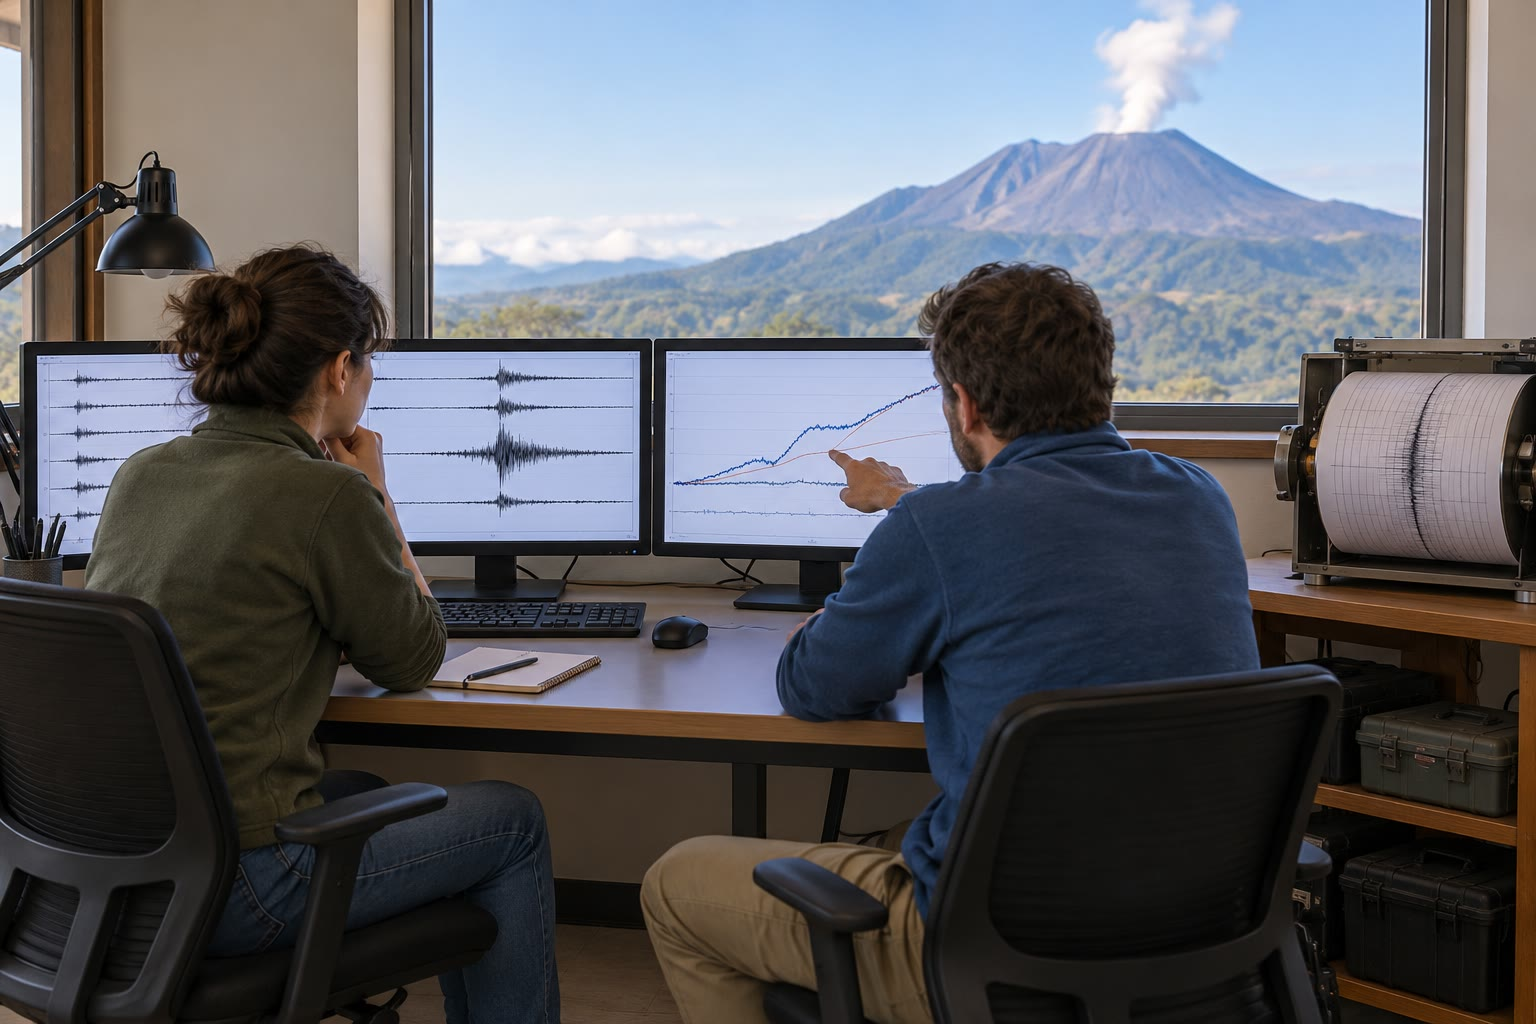
\includegraphics[width=\linewidth]{images/book4/ai/b2-volcano-observatory.jpg}
\par\smallskip{\scriptsize Wetenschappers bekijken seismische registraties in een
vulkaanobservatorium (door AI gegenereerde illustratie).}
\end{minipage}
\end{inthefield}
% ledger: hvo:alert-levels

\section{Oefeningen}

\begin{exercise}[$\star$]\label{exo:b2:eruptive-styles:1}
Geef de VEI die alleen al uit het bulkvolume \omterm{def:b2:eruptive-styles:tephra}{tefra} volgt voor: (a) de as van
Mount St.~Helens, 18 mei 1980, \qty{1.3}{km^3}; (b) de valafzetting Laag~5 van de Cotopaxi,
\qty{0.29}{km^3}; (c) een kleine eruptie van \qty{2e6}{m^3}. (d) Het materiaal
dat de Pinatubo in 1991 uitwierp, wordt opgegeven als ``meer dan \qty{5}{km^3}'', maar de
eruptie krijgt VEI~6. Welk bulkvolume houdt die waardering minstens in?
\end{exercise}
% ledger: usgs:vei-criteria, usgs:msh-1980-ash, biass19:layer5, usgs:pinatubo-1991

\begin{exercise}[$\star$]\label{exo:b2:eruptive-styles:2}
Benoem elke \omterm{def:b2:eruptive-styles:tephra}{pyroclast}: (a) een glasscherf van \qty{0.5}{mm} lang; (b) een
puimsteenfragment van \qty{3}{cm} doorsnede; (c) een hoekig stuk oude lava van \qty{20}{cm}
doorsnede; (d) een spoelvormige klont van \qty{8}{cm} lang met gedraaide uiteinden.
\end{exercise}
% ledger: nps:pyroclast-sizes

\begin{exercise}[$\star$]\label{exo:b2:eruptive-styles:3}
Met $H = 0.304\,Q^{0.241}$ ($H$ in kilometer boven de krater, $Q$ in
\unit{kg/s}): (a) bereken $H$ voor $Q = \qty{e6}{kg/s}$ en \qty{e8}{kg/s};
(b) bereken het massadebiet dat een kolom van \qty{35}{km} hoog inhoudt, en zijn
intensiteit $I = \log_{10}Q + 3$; (c) met welke factor verandert $Q$ als de gemeten
hoogte \qty{20}{\percent} te hoog is?
\end{exercise}
% ledger: aubry23:fits, brown14:record

\begin{exercise}[$\star$]\label{exo:b2:eruptive-styles:4}
De valafzetting Laag~5 van de Cotopaxi heeft een bulkvolume van \qty{0.29}{km^3}. Bereken, met een
bulkdichtheid van \qty{1000}{kg/m^3} voor de afzetting en \qty{2500}{kg/m^3} voor het
\omterm{def:b2:magma-emplacement:magma}{magma}, haar volume als equivalent in dicht gesteente, haar massa en haar magnitude
$M = \log_{10}m - 7$.
\end{exercise}
% ledger: biass19:layer5, brown14:record

\begin{exercise}[$\star\star$]\label{exo:b2:eruptive-styles:5}
Een valafzetting is \qty{40}{cm} dik op de isopach van $\sqrt A = \qty{5}{km}$
en \qty{10}{cm} op die van $\sqrt A = \qty{15}{km}$, en wordt dunner als één enkele
exponentiële. Bereken $k$, $T_0$, de halveringsafstand van de dikte $\ln 2/k$, het
bulkvolume en de VEI.
\end{exercise}

\begin{exercise}[$\star\star$]\label{exo:b2:eruptive-styles:6}
(a) Toon aan dat het volume binnen de isopach $x = \sqrt A$ van een afzetting die dunner wordt
als $T_0e^{-kx}$, gelijk is aan $\frac{2T_0}{k^2}[1 - (1 + kx)e^{-kx}]$. (b) Los $(1 + u)e^{-u} =
1/2$ op tot op drie beduidende cijfers met herhaalde substitutie of bisectie. (c) Voorbij welke isopach ligt
voor de afzetting van \cref{exo:b2:eruptive-styles:5} de helft van het volume? Vergelijk
met de afstand tot de krater van de buitenste isopach die in kaart is gebracht.
\end{exercise}

\begin{exercise}[$\star\star$]\label{exo:b2:eruptive-styles:7}
Een rhyolitisch \omterm{def:b2:magma-emplacement:magma}{magma} van \qty{850}{\celsius} (\qty{1123}{K}) bevat
\qty{5.0}{\percent} water, met oplosbaarheid $s = 0.444$ procent per
$\sqrt{\unit{MPa}}$; zijn smelt heeft een dichtheid van \qty{2300}{kg/m^3}. (a) Bereken zijn
verzadigingsdruk, en de diepte waarop die wordt bereikt bij een drukgradiënt
van \qty{0.025}{MPa/m}. (b) Bereken de gasvolumefractie bij
\qty{10}{MPa} als het gas in het \omterm{def:b2:magma-emplacement:magma}{magma} blijft ($R = \qty{8.314}{J/(mol.K)}$, $M =
\qty{0.018015}{kg/mol}$). (c) Waarom fragmenteren basaltische \omterm{def:b2:magma-emplacement:magma}{magma's} zoveel minder
vaak, hoewel een basalt in een gesloten systeem met \qty{1}{\percent} water bij \qty{1}{MPa}
voor \qty{92}{\percent} uit gas zou bestaan?
\end{exercise}
% ledger: moore98:h2o, cassidy18:fragmentation, cassidy18:ascent

\begin{exercise}[$\star\star$]\label{exo:b2:eruptive-styles:8}
(a) Een \omterm{prop:b2:eruptive-styles:mogi}{mogibron} op \qty{5}{km} diepte groeit met \qty{e7}{m^3}. Bereken de
opheffing erboven ($\nu = 0.25$). (b) Een andere bult daalt tot de helft van zijn maximum
op \qty{3.8}{km} van zijn centrum: hoe diep ligt zijn bron? (c) Welke fractie van de
maximale opheffing ziet een station op een horizontale afstand gelijk aan de diepte van de
bron?
\end{exercise}
% ledger: dmodels:mogi

\begin{exercise}[$\star\star$]\label{exo:b2:eruptive-styles:9}
Een Vulcanische explosie werpt blokken uit een krater. Bereken, zonder luchtweerstand
en zonder de hoogte van de kraterrand, de grootste dracht van een blok dat wordt gelanceerd
met \qty{100}{m/s}, daarna met \qty{200}{m/s} ($g = \qty{9.81}{m/s^2}$). Maakt de
luchtweerstand van deze drachten een boven- of een ondergrens? Waarom schaalt een zone van
ballistisch gevaar rond een krater met het kwadraat van de lanceersnelheid?
\end{exercise}

\begin{exercise}[$\star\star\star$]\label{exo:b2:eruptive-styles:10}
(a) Leid het volume af van een afzetting met twee exponentiële segmenten dat in het
methodekader wordt gegeven, in de veronderstelling dat de dikte continu is waar de lijnen elkaar snijden. (b) Voor
de valafzetting Laag~5 van de Cotopaxi zijn de gefitte segmenten $T = \qty{1285}{cm}\times
e^{-0.365x}$ en een distaal segment met helling $k_2 = \qty{0.138}{km^{-1}}$, die elkaar snijden bij
$X = \qty{8.56}{km}$. Bereken het volume, en het aandeel ervan voorbij het
snijpunt.
\end{exercise}
% ledger: biass19:layer5

\begin{exercise}[$\star\star\star$]\label{exo:b2:eruptive-styles:11}
(a) Met welke factor stijgt, volgens \cref{prop:b2:eruptive-styles:plume}, de hoogte van een
kolom als het eruptiedebiet met 100 wordt vermenigvuldigd? Vergelijk met de
empirische exponenten $0.241$ en $0.226$. (b) Hoe verandert een sterker
gelaagde atmosfeer de hoogte, en met hoeveel als $N$ met
\qty{20}{\percent} groeit? (c) Geef twee redenen waarom gemeten exponenten onder
$1/4$ kunnen uitvallen.
\end{exercise}
% ledger: aubry23:fits

\begin{exercise}[$\star\star\star$]\label{exo:b2:eruptive-styles:12}
De wereldwijde catalogus telt 132 erupties van VEI~4 of meer die begonnen tussen 1500
en 1899, en 95 tussen 1900 en 2024. (a) Bereken de frequentie per eeuw in elke
periode. (b) Als de frequentie sinds 1900 de ware is, welke fractie van de eerdere
erupties werd dan opgetekend? (c) Een studie van grote erupties vindt 21 erupties van
magnitude 4 tot 4.9 per eeuw tussen 1500 en 1900 en 56 sinds 1900; vergelijk.
(d) Waarom hangt deze fractie af van de grootte van de erupties?
\end{exercise}
% ledger: data:b4-gvp-eruptions, brown14:record

\section{Probleem: Een Plinische afzetting lezen}

\begin{problem}[{Weekendprobleem --- van de isopachen van een puimsteenafzetting naar de grootte
van haar eruptie, de hoogte van haar kolom, en hoe vaak zulke erupties
voorkomen}]
\label{pb:b2:eruptive-styles:1}
Een denkbeeldige vulkaan heeft een puimsteenafzetting achtergelaten uit één enkele Plinische fase die
\qty{10}{\hour} duurde. Haar isopachen, nadat de uitrekking door de wind is weggewerkt door
de vierkantswortel van hun oppervlakten te gebruiken, zijn:
\begin{center}
\small
\begin{tabular}{lccccc}
\hline
$\sqrt A$ (\unit{km}) & 10 & 20 & 40 & 80 & 120 \\
dikte $T$ (\unit{cm}) & 200 & 100 & 48 & 14 & 4.0 \\
\hline
\end{tabular}
\end{center}
Gegevens: bulkdichtheid van de afzetting \qty{900}{kg/m^3}; dichtheid van het \omterm{def:b2:magma-emplacement:magma}{magma}
\qty{2400}{kg/m^3}; kolomhoogte gemeten uit de grootste klasten,
\qty{31}{km} boven de krater; tropopauze op \qty{16}{km}. Gebruik $H =
0.304\,Q^{0.241}$ en $H = 0.345\,Q^{0.226}$ ($H$ in kilometer, $Q$ in
\unit{kg/s}).

\medskip\noindent\textbf{Deel I --- De afzetting.}
\begin{enumerate}
\item Bereken $\ln T$ voor elke isopach en toon aan dat de punten op twee
rechte segmenten vallen als ze tegen $\sqrt A$ worden uitgezet. Waar ligt de knik?
\item Bereken de helling $k_1$ en het snijpunt met de as $T_0$ van het proximale segment
door de eerste twee isopachen.
\item De kleinste-kwadratenrechte door de drie distale isopachen is $T =
\qty{167}{cm}\times e^{-0.0311\sqrt A}$. Controleer dat ze binnen
\qty{5}{\percent} van elk ervan ligt.
\item Bereken de waarde van $\sqrt A$ waarbij de twee lijnen elkaar snijden.
\item Bereken de halveringsafstanden van de dikte $\ln 2/k$ van de twee segmenten.
\item Bereken het volume dat de afzetting zou hebben als ze overal met de proximale
helling dunner werd.
\item Bereken het bulkvolume met de twee segmenten, en het aandeel van
de correctie voor het flauwere distale segment.
\item Met welke factor zou het volume worden onderschat als alleen de proximale
afzetting in kaart was gebracht? Waarom is dat een reëel risico voor oude afzettingen?
\end{enumerate}

\noindent\textbf{Deel II --- De grootte van de eruptie.}
\begin{enumerate}[resume]
\item Geef de VEI van de eruptie.
\item Bereken het volume als equivalent in dicht gesteente.
\item Bereken de uitgeworpen massa.
\item Bereken de magnitude $M = \log_{10}m - 7$.
\item Hoeveel keer groter dan de asval van Mount St.~Helens in 1980,
\qty{1.3}{km^3}, is deze afzetting?
\item Welke kolomhoogte verbindt de VEI-tabel met deze eruptie, en
welke stijl?
\end{enumerate}

\noindent\textbf{Deel III --- De kolom.}
\begin{enumerate}[resume]
\item Bereken het gemiddelde massadebiet over de Plinische fase, en zijn
intensiteit $I = \log_{10}Q + 3$.
\item Bereken de kolomhoogte die de eerste empirische wet voorspelt.
\item Hetzelfde met de tweede wet.
\item Vergelijk met de \qty{31}{km} die uit de klasten is gemeten, gezien de spreiding
van de wetten.
\item Welk massadebiet zou \qty{31}{km} volgens de eerste wet inhouden? Met welke
factor verschilt het van dat van vraag~15, en wat zou dat kunnen verklaren?
\item Bracht de kolom gas in de stratosfeer? Wat zou er voor het
klimaat kunnen volgen, en wat zou het sleutelgas zijn?
\end{enumerate}

\noindent\textbf{Deel IV --- Hoe vaak?}
\begin{enumerate}[resume]
\item Bereken uit de tellingen van de catalogus (399 erupties van VEI $\ge 3$ van 1950 tot
2024, 95 van VEI $\ge 4$ vanaf 1900, 22 van VEI $\ge 5$ vanaf 1800, 8 van VEI $\ge 6$ vanaf
1500, alle vensters eindigend in 2024, dat jaar inbegrepen) de vier jaarlijkse frequenties en
hun logaritmen.
\item Controleer dat de rechte $\log_{10}\lambda_v = 3.28 - 0.85\,v$ binnen
\qty{10}{\percent} van elke frequentie ligt.
\item Waarom begint elk venster verder terug voor grotere erupties?
\item Bereken uit de rechte de frequentie van erupties van VEI $\ge 5$, hun gemiddelde
herhalingstijd, en de kans op minstens één in de komende 10 jaar.
\item Bereken uit de rechte de frequentie van erupties van VEI $\ge 7$ en vergelijk ze
met de twee die sinds het jaar 1000 zijn opgetekend.
\item Bereken uit de rechte de frequentie van erupties van VEI $\ge 6$ en de
kans, in procent, op minstens één ergens op aarde in de komende 100
jaar, het kerngetal van dit probleem. Op welke aanname berust ze?
\end{enumerate}
\end{problem}
